\documentclass[12pt]{article}
\usepackage[]{graphicx}
\usepackage[]{color}
\usepackage[top=1in,left=1in, right = 1in, footskip=1in]{geometry}

\title{Speed and strength of an epidemic intervention}
\author{Jonathan Dushoff, Sang Woo Park}

\usepackage{tabularx}

%% \usepackage{amsmath}
\usepackage{natbib}
\usepackage{hyperref}
\bibliographystyle{chicago}
\date{\today}

\usepackage{bm}

\usepackage{afterpage}
\usepackage{pdflscape}

\newcommand{\etal}{\textit{et al.}}

\newcommand{\comment}[3]{\textcolor{#1}{\textbf{[#2: }\textit{#3}\textbf{]}}}
\newcommand{\jd}[1]{\comment{cyan}{JD}{#1}}
\newcommand{\swp}[1]{\comment{magenta}{SWP}{#1}}

\newcommand{\Rx}[1]{\ensuremath{{\mathcal R}_{#1}}} 
\newcommand{\Ro}{\Rx{0}}
\newcommand{\RR}{\ensuremath{{\mathcal R}}}
\newcommand{\Rhat}{\ensuremath{{\hat\RR}}}
\newcommand{\tsub}[2]{#1_{{\textrm{\tiny #2}}}}
\newcommand{\pEarly}{\ensuremath{\tsub{p}{early}}}

\newcommand{\figref}[1]{Fig.~\ref{fig:#1}}
\newcommand{\figlab}[1]{\label{fig:#1}}
\newcommand{\eqref}[1]{(\ref{eq:#1})}
\newcommand{\eqlab}[1]{\label{eq:#1}}
\begin{document}

\maketitle

\section*{Abstract}

While an epidemic can be characterized by its speed (i.e., the exponential growth rate $r$) and strength (i.e., the reproductive number \RR), the effectiveness of an intervention strategy is often, if not always, determined by its ability to reduce \RR\ below 1.
Here, we generalize this idea by measuring the speed and strength of intervention on the same scale as the speed and strength of an epidemic, respectively.
We show that an epidemic can be contained if the speed or strength of intervention is greater than their corresponding counterparts.
Finally, we compare two intervention strategies for HIV -- namely condom intervention and test-and-treat intervention -- to demonstrate that both speed- and strength-based perspectives can be useful for evaluating intervention strategies under different scenarios.
We suggest that disease modelers should refrain from putting too much emphasis on the reproductive number but rather consider both speed- and strength-based perspectives.

\section{Introduction}

An epidemic can be described by its \emph{speed} and \emph{strength}.
The speed of an epidemic is characterized by the exponential growth rate $r$, which measures how \emph{fast} an epidemic grows at the population level.
The strength of an epidemic is characterized by the reproductive number \RR, which measures how many new cases are caused by a typical \emph{individual} case.
Knowing the speed and strength of an epidemic allows predictions about the course of the epidemic and the effectiveness of intervention strategies.

Much research has prioritized estimates of \RR, and particularly its value in a fully susceptible population, called the \emph{basic} reproductive number \Ro, because \RR\ has a threshold value (i.e., $\RR=1$) that determines whether a disease can invade, the level of equilibrium, and the effectiveness of control efforts \citep{anderson1991infectious, diekmann1990definition}.
The insight that a case must on average cause at least one new case under good conditions for a disease to persist goes back $>100$ years \citep{ross1911prevention};
the idea of averaging by defining a `typical' case was formalized 30 years ago \citep{diekmann1990definition}.
$\RR$ is also of interest because it provides a \emph{prima facie} prediction about the total \emph{size} of an epidemic \citep{anderson1991infectious, ma2006generality, arino2007final, andreasen2011final, miller2012note}.

Here, we generalize the idea of a threshold for successful intervention by measuring an intervention's ``strength'' on the same scale as the reproductive number. 
We then show that we can likewise measure an intervention's ``speed'', and that there is a duality between the threshold $\RR=1$ and a corresponding minimal intervention strength required for elimination, and the threshold $r=0$ and a corresponding minimal intervention speed. 
We argue that the historical primacy of $\RR$ over $r$ is partly artificial, and discuss cases where strength provides the better framing for practical disease questions and cases where speed does.

\section{Methods}

\subsection{Epidemic model}

We model disease incidence using the renewal equation, a simple, flexible framework that can cover a wide range of model structures \citep{heesterbeek1996concept, diekmann2000mathematical, roberts2004modelling, aldis2005integral, wallinga2007generation, roberts2007model, Champredon2018equivalence}.
In our model, disease incidence at time $t$ is given by:
\begin{equation}
i(t) = \int K(\tau, t) i(t-\tau) d\tau.
\end{equation}
Here, $K(\tau, t)$ is the infection kernel describing how infectious we expect an individual infected $\tau$ time units ago to be in the population.
In general, $K(\tau, t)$ will depend on population characteristics that may change through time $t$ -- notably, the proportion of the population susceptible, $S(t)$.
Since we are interested in invasion and control, we will generally neglect changes in $K(\tau, t)$ through time.
Thus, we will assume $K(\tau, t) \equiv K(\tau)$.
Importantly, this means we are neglecting changes in susceptible proportion through time: $S(t) \approx S(0)$.
Under this assumption, the renewal equation is equivalent to the Von Foerster equations (see e.g. \cite{fraser2004factors}).

\subsection{Strength-based decomposition}


\begin{figure}[!t]
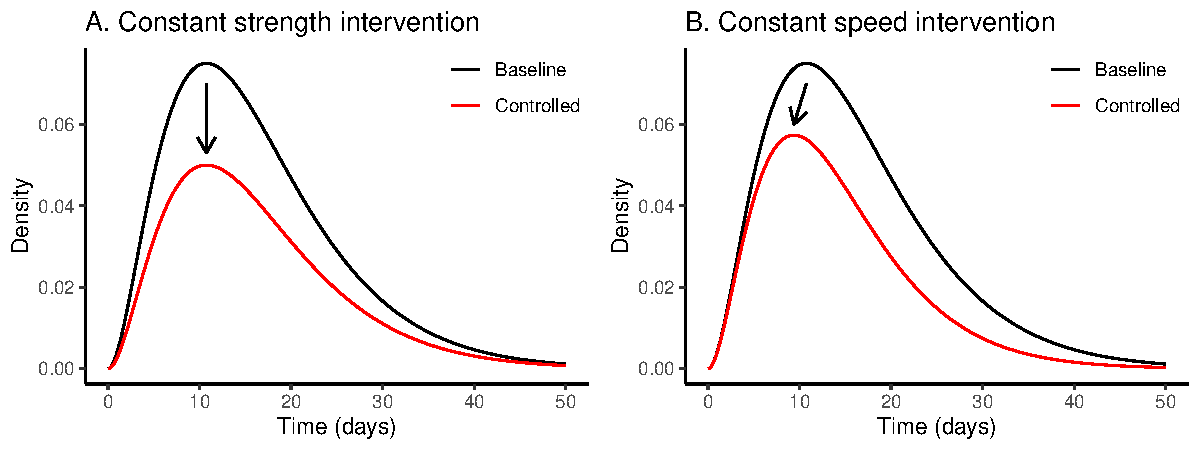
\includegraphics[width=\textwidth]{../figure/constant_intervention.pdf}
\caption{
\textbf{Effects of constant-strength and constant-speed intervention on infection kernels.}
Ebola-like gamma infection kernel $K(\tau)$ (mean: 16.2 days, CV: 0.58, and \Ro: 1.5) is shown in black \citep{park2019practical}.
The infection kernel after applying each intervention strategy $\hat K(\tau)$ is shown in red.
(A) The effect of a constant-strength intervention with $\theta = 1.5$.
A constant-strength intervention reduces the density by a constant proportion: $\hat K(\tau) = K(\tau)/\theta$; when the strength of intervention matches the strength of epidemic ($\theta = \mathcal R$), the resulting distribution is equivalent to the intrinsic generation-interval distribution ($\hat K(\tau) = g(\tau)$).
(B) A constant-speed intervention with $\phi \approx 0.0267/\mathrm{day}$ is applied to the same kernel.
A constant-speed intervention reduces the density exponentially: $\hat K(\tau) = K(\tau) \exp(-\phi \tau)$; when the speed of intervention matches the speed of epidemic ($\phi = r$), the resulting distribution is equivalent to the initial backward generation-interval distribution ($\hat K(\tau) = b(\tau)$). 
}
\figlab{constant}
\end{figure}

Assuming that the infection kernel $K$ doesn't change with time, we write:
\begin{equation}
	K(\tau) = \RR g(\tau),
	\eqlab{strengthFactors}
\end{equation}
where $g(\tau)$ is the ``intrinsic'' generation-interval distribution.
The generation interval is defined as the time between when a person becomes infected and when that person infects another person \citep{svensson2007note};
therefore, the intrinsic generation-interval distribution $g(\tau)$ gives the relative infectiousness of an average individual as a function of time since infection \citep{champredon2015intrinsic}. 
Since $g$ is a distribution, it integrates to 1, and the basic reproductive number $\RR$ is thus the integral of $K$.

Imagine a control measure that proportionally reduces $K$, for example, by protecting a fixed fraction of susceptibles through vaccination (\figref{constant}A). We then have:
\begin{equation}
	\hat K(\tau) = (\RR/\theta) g(\tau).
\end{equation}
Since $g$ is a distribution, the reduction needed to prevent invasion (or to eliminate disease)  is exactly $\theta=\RR$. We call $\theta$ the ``strength'' of the intervention; transmission is interrupted when the strength of the intervention $\theta$ is larger than the strength of spread $\RR$.

We generalize this idea by allowing an intervention strategy to reduce $K$ by different proportions over the course of an individual infection. We write the post-intervention kernel:
\begin{equation}
	\hat K(\tau) = K(\tau)/L(\tau), 
\end{equation}
where $L(\tau)$ is the average proportional reduction for an individual infected time $\tau$ ago.
The post-intervention reproductive number is thus:
\begin{equation}
	\Rhat = \int \hat K(\tau) d\tau
\end{equation}
This framework generalizes the work of \cite{fraser2004factors} who made parametric assumptions about the shape of $L(\tau)$. 

We define the strength of the intervention $L$ to be $\theta = \RR/\Rhat$. It is then straightforward to show that $\theta$ is the harmonic mean of $L(\tau)$ weighted by generation-interval distribution:
\begin{equation}
	\theta = 1/\langle 1/L(\tau) \rangle_{g(\tau)}.
	\eqlab{strengthMean}
\end{equation}
In this more general case, we have again that the disease cannot spread when $\theta \geq \RR$.

\subsection{Speed-based decomposition}

The Euler-Lotka equation allows us to calculate the initial exponential growth rate $r$ of an epidemic given an infection kernel $K$:
\begin{equation}
	1 = \int K(\tau) \exp(-r\tau) d\tau
	\eqlab{euler}
\end{equation}
By analogy with the strength-based factorization \eqref{strengthFactors}, we can rewrite \eqref{euler} as a speed-based factorization:
\begin{equation}
K(\tau) = b(\tau)\exp(r\tau)
\end{equation}
Like $g$, $b$ is a distribution: in this case the initial backward generation interval, which gives the distribution of realized generation times (measured from the infectee's point of view) when the disease spreads exponentially \citep{champredon2015intrinsic, britton2019estimation}.

Now imagine an intervention that reduces transmission at a constant hazard rate $\phi$ across the disease generation (\figref{constant}B), for example, by identifying and isolating infectious individuals.
We then have:
\begin{equation}
	\hat K(\tau) = K(\tau)\exp(-\phi\tau) = b(\tau)\exp((r-\phi)\tau)
\end{equation}
Since $b$ is a distribution (which integrates to 1), the reduction needed to prevent invasion (or to eliminate disease)  is exactly $\phi=r$. 
We call $\phi$ the ``speed'' of the intervention; transmission is interrupted when the speed of the intervention is faster than the speed of spread.

We generalize this idea by allowing the hazard rate $h(\tau)$ at which $K$ is reduced to vary through time, thus:
\begin{equation}
	\hat K(\tau) = K(\tau) \exp\left(-\int_0^\tau h(\sigma) d\sigma\right)
\end{equation}
The associated post-intervention epidemic speed $\hat r$ is given by:
\begin{equation}
	1 = \int \hat K(\tau) \exp(-\hat r\tau) d\tau.	
\end{equation}
We define the speed of a general intervention to be $\phi = r - \hat r$. 
We can then show that $\phi$ is a (sort of) mean satisfying the implicit equation:
\begin{equation}
	1 = \left\langle \frac{\exp(\phi \tau) }{\exp\left(\int_0^\tau h(\sigma) d\sigma\right)} \right\rangle_{b(\tau)}
	\eqlab{speedMean}
\end{equation}
Specifically, the speed $\phi$ is a mean of the hazard $h$ in the sense that an increase (or decrease) in $h$ produces the same sign of change in $\phi$, and if $h$ is constant across the generation then $\phi=h$.

\section{Example: Human immunodeficiency virus (HIV)}

In this section, we use both strength- and speed-based decompositions to compare different intervention strategies for the human immunodeficiency virus (HIV). 
In particular, we study how the amount of early HIV transmission affects estimates of intervention effectiveness. 
These examples are not detailed estimates for specific scenarios; 
instead, they are meant to demonstrate how strength- and speed-based decompositions can help evaluate control strategies.

We model the infection kernel of the HIV as a sum of two gamma distributions:
\begin{equation}
K(\tau) = \mathcal R \left(\tsub{p}{early} \tsub{f}{early}(\tau) + (1-\tsub{p}{early}) \tsub{f}{late}(\tau) \right).
\end{equation}
The first component, $\tsub{f}{early}(\tau)$, models early HIV transmission during the acute infection stage.
We assume that $\tsub{f}{early}(\tau)$ has a mean of 3 months \citep{hollingsworth2008hiv} and a shape parameter of 3.
The second component, $\tsub{f}{late}$, models HIV transmission during the asymptomatic stage and the disease stage (after progression to Acquired Immune Deficiency Syndrome (AIDS)).
We assume that $\tsub{f}{late}(\tau)$ has a mean of 10 years \citep{brookmeyer1989censoring, nishiura2019estimating} and a shape parameter of 2 (this vaguely approximates the wide generation-interval distribution of the HIV \citep{fraser2004factors}).
Finally, $\tsub{p}{early}$ is the proportion of early HIV transmission.

\begin{figure}[!th]
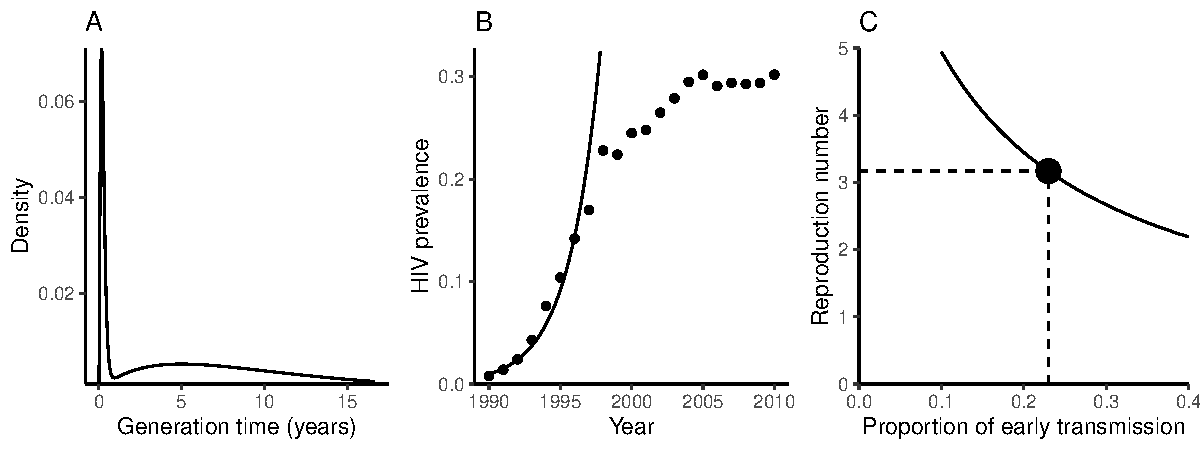
\includegraphics[width=\textwidth]{../figure/HIV.pdf}
\caption{
\textbf{The infection kernel of the HIV.}
(A) The infection kernel of the HIV is approximated using a sum of two gamma distributions. We assume that the baseline proportion of early transmission is 23\% \citep{hayes2006amplified}.
(B) Time series of HIV prevalence in pregnant women in South Africa, 1990 - 2010 \citep{barron2013eliminating}. The initial exponential growth rate of the HIV is estimated by fitting a straight line to log-prevalence (1990 - 1997) by minimizing the sum of squares.
(C) Increase in the estimate of the amount of early transmission reduces the estimate of the reproductive number.
The black circle indicates the baseline scenario.
}
\figlab{example}
\end{figure}

The infection kernel is shown in (\figref{example}A) for our baseline value of  
$\tsub{p}{early} = 0.23$.  We assume that the initial speed of the epidemic is $r=0.452\,\mathrm{year}^{-1}$(\figref{example}B), and ask what value of $\Ro$ would produce this rate of growth.
When transmission is fast, (i.e., when \pEarly\ is large), individuals don't need to transmit as much to achieve this speed, so the estimated value of \Ro\ decreases (\figref{example}C).
Therefore, as \pEarly\ gets smaller, we expect stronger intervention to be required in order to control the disease.

We compare two different possible intervention strategies to shed light on the speed and strenght decompositions.
First, we consider a condom intervention that reduces HIV transmission by approximately 75\% at the population level.
Assuming that condoms act as a physical barrier, and that condom use will, on average, remain roughly constant through time, it is reasonable to model the proportional reduction in transmission due to condom use as constant across the course of infection: $\tsub{L}{condom} = 1/(1-0.75) = 4$  (\figref{condom}A).
The estimated strength of such an intervention is simply the average of $\tsub{L}{condom}$, i.e., $\theta=4$, whereas the estimated strength of the epidemic decreases as the proportion of early transmission increases (\figref{condom}B).
Thus, the predicted effectiveness of the condom intervention will depend strongly on our estimate of the importance of early transmission: if early transmission is low, we expect disease spread to be too strong to be controlled completely by our intervention.

\begin{figure}[!t]
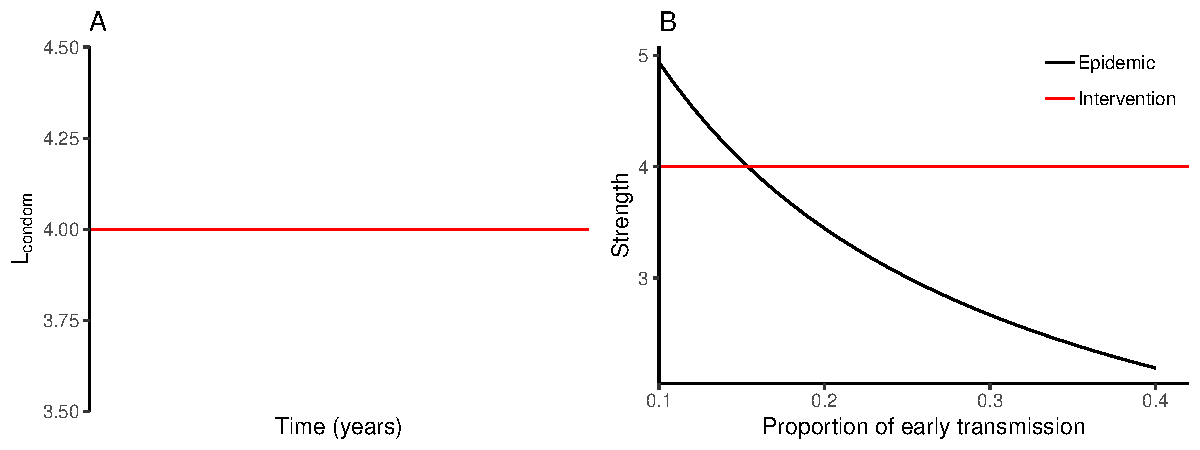
\includegraphics[width=\textwidth]{../figure/condom.pdf}
\caption{
\textbf{Understanding condom intervention using strength-based decomposition.}
(A) Condom use is thought to reduce probability of transmission by a similar factor throughout the course of infection; thus the proportional reduction $\tsub{L}{condom}$ due to condom use is constant across the course of infection.
(B) The estimated amount of early transmission affects estimated strength of the epidemic but not of a condom-based intervention.
The black and red circles indicate the baseline scenario.
}
\figlab{condom}
\end{figure}


\begin{figure}[!t]
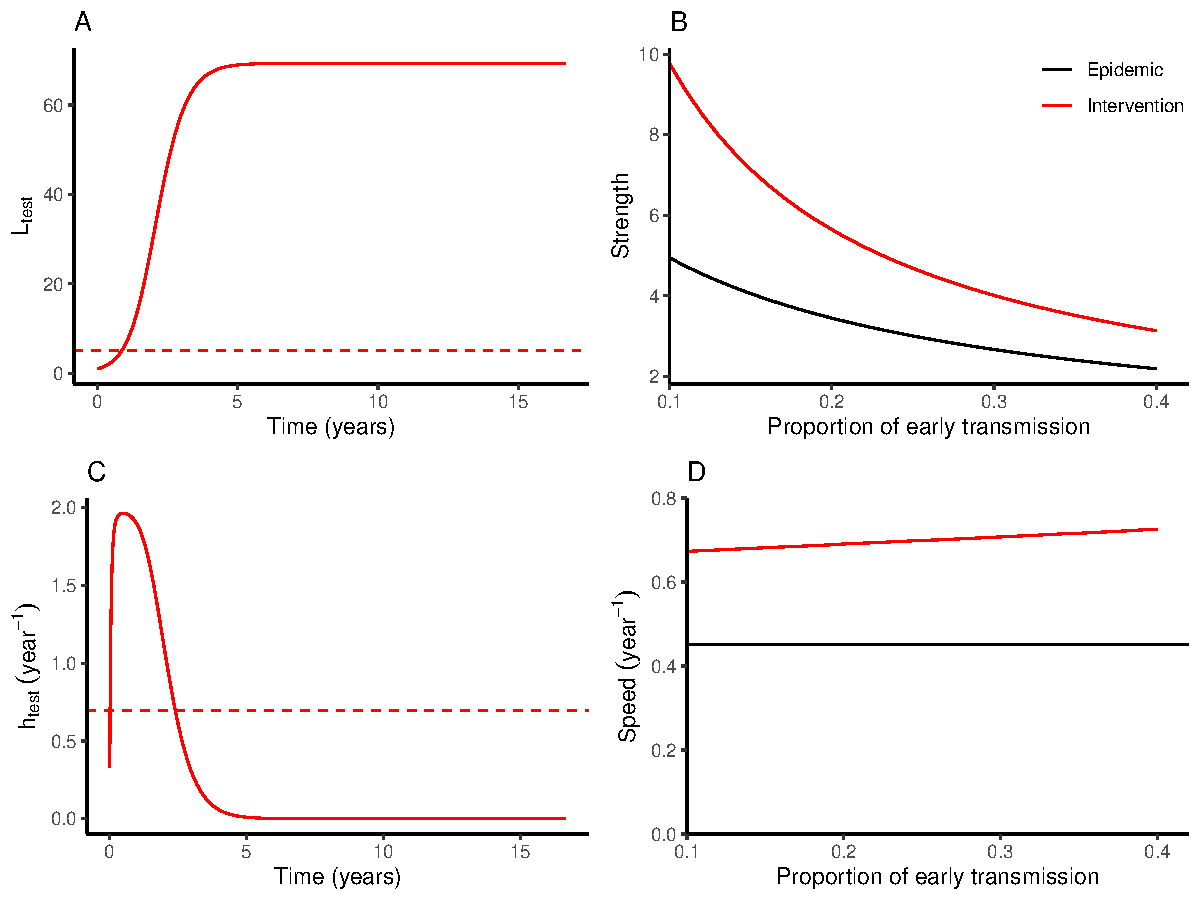
\includegraphics[width=\textwidth]{../figure/test_and_treat.pdf}
\caption{
\textbf{Understanding test-and-treat intervention using strength- and speed-based decomposition.}
(A) The strength of the test-and-treat intervention (calculated from the assumed hazard, (C)). The dashed line shows the corresponding effective strength of the intervention (from \eqref{strengthMean}) assuming 23\% early transmission.
(B) Increase in the estimated amount of early transmission decreases the estimated strength of an epidemic as well as the estimated strength of test-and-treat intervention.
(C) The assumed hazard for the test-and-treat intervention. 
The dashed line shows the corresponding effective speed of the intervention (from \eqref{speedMean}) assuming 23\% early transmission.
(D) The estimated amount of early transmission has little effect on the effective speed of intervention, and none on the speed of the epidemic estimated from incidence data.
Circles indicate the baseline scenario.
Test-and-treat intervention is modeled phenomenologically: $\tsub{L}{test}(\tau) = \exp\left(\int_0^\tau \tsub{h}{test}(\sigma) d\sigma \right)$ and $\tsub{h}{test}(\tau) = \tsub{h}{max} (1 - \exp(- K f(\tau)))$, where $f(\tau)$ is a gamma probability density function with a mean of $1$ year and a shape parameter of 2, $K = 4/\max(f(\tau))$, and $\tsub{h}{max} = 2\,\mathrm{year}^{-1}$.
}
\figlab{test}
\end{figure}

On the other hand, consider a ``test-and-treat'' strategy in which infected individuals are identified and put to clinical care, such as antiretroviral therapy (ART) \citep{garnett2009treating, nah2017test}.
We assume that the rate of identification and removal is initially constant.
Thus, the proportion continuing to transmit declines exponentially, and the effect of intervention $\tsub{L}{test}$ increases exponentially.
However, we assume removal eventually saturates, to account for the effects of people who avoid identification, persistent treatment failures, and the possibility of rare transmission even under effective treatment
(\figref{test}A; see caption for the functional form of $\tsub{L}{test}$).
Under this assumption, the strength of intervention decreases with the proportion of early transmission in a manner roughly similar to the epidemic strength.
In this scenario, we predict that the intervention remains effective over the range of considered parameters.

Using the speed-based decomposition provides a valuable perspective on this situation.
The hazard rate $\tsub{h}{test}$ of this intervention starts at 0 (because infected individuals don't have a way to know that they have HIV when they're infected) but peaks very fast (because sexually active individuals are the most likely to seek testing); 
the assumed hazard rate goes down after a few months to reflect the saturation assumptions discussed above. 
The estimated epidemic speed depends only on the observed growth rate -- it does not change if we change our assumption about the proportion of early transmission.
The effective speed of the intervention stays relatively constant, in part because the backward generation-interval distributions for different  scenarios are relatively similar.
The intervention speed increases slightly as proportion of early transmission increases because the subpopulation that the intervention fails to reach become relatively more important if late transmission is more important.
This framework provides an intuitive underpinning for the originally surprising result of \cite{eaton2014proportion}: the effectiveness of test-and-treat interventions should not depend much on the proportion of early transmission because early transmission has no effect on the estimated speed of the epidemic, and little on the estimated speed of the intervention.

\section{Discussion}

The effectiveness of an epidemic intervention is often measured by its ability to reduce the reproductive number -- \RR, or outbreak ``strength'' -- below 1. The exponential growth rate -- $r$, or outbreak ``speed'' -- is often seen just as a stepping stone to \RR\, or even overlooked entirely \citep{park2020reconciling}.
We argue that \RR\ and $r$ provide equally valid, complementary perspectives on epidemic control, and that there are situations where each provides a clearer picture than the other.

In this study, we:
first extended the standard paradigm of \RR\ as critical parameter for control, by defining the strength of an intervention on the same scale as \RR, the strength of the epidemic; 
then constructed a parallel interpretation which measures the speed of an intervention on the same scale as $r$, the speed of an epidemic.
We thus showed that the standard paradigm for \RR\ and control has a natural parallel interpretation in terms of $r$.

To illustrate this idea, we used simple assumptions to explore the effects of two HIV intervention strategies (condoms and test-and-treat), using both strength- and speed-based frameworks.
In particular, we provided an alternative explanation for the result of \cite{eaton2014proportion} who used detailed mathematical modeling of HIV transmission to show that the amount of early transmission does not affect the effectiveness of the ART:
we can control an outbreak if we can identify infected individuals and enroll them on ART faster than the \emph{observed} rate at which new cases are generated, which does not depend on the estimates of the amount of early transmission.
The original explanation of the result relied on a strength-based arugment: increasing the amount of early transmission decreases the basic reproductive number, which negatively correlates with the outcome of the ART intervention \citep{eaton2014proportion}.

While both speed- and strength-based frameworks give the same conclusion about the outcome of an intervention, one can provide a clearer interpretation of the outcome than the other.
Which is more appropriate depends on disease dynamics as well as intervention strategies.
We expect the speed-based framework to be better at characterizing newly invading pathogens and evaluating intervention strategies that seek to slow down transmission at the individual-level:
when an epidemic is growing exponentially, the reproductive number cannot be estimated with confidence \citep{weitz2015modeling}, especially when there is large uncertainty in the shape of the generation-interval distribution \citep{park2020reconciling},
whereas the exponential growth rate can be directly measured from incidence curves \citep{ma2014estimating}.
On the other hand, we expect the strength-based framework to be better for characterizing endemic diseases and evaluating intervention strategies that seek to reduce the overall transmission at the population-level:
(i) the endemic equilibrium is determined by the reproductive number and (ii) the long-term outcomes of vaccine-like interventions are typically independent of how fast the intervention is implemented.
There are also cases where both speed- and strength-based perspectives are equally important:
controlling an outbreak via active-vaccination requires rapid distribution (speed-like) of efficacious vaccine (strength-like).

The contrast between speed- and strength-based perspectives can be found in other literature as well.
For example, whether the instantaneous per capita rate of increase $r$ (speed) or expected life time reproductive success $R_0$ (strength) is the correct measures of fitness depends on the mechanism of density dependence \citep{pasztor1996r0}.
When population is regulated by affecting all individuals identically, $r$ is a valid measure \citep{pasztor1996r0}.
When population is regulated by affecting density-dependent juvenile mortality, $R_0$ is a valid measure \citep{mylius1995evolutionarily}.
Even though the contrast between the strength- and speed-based perspectives was formalized in theoretical ecology more than 20 years ago, it is still rare in theoretical epidemiology.

Responses to the 2014 Ebola Outbreak in West Africa and the recent COVID-19 outbreak clearly demonstrate the lack of emphasis on the speed of an epidemic.
During the early phases of both outbreaks, many disease modelers tried to estimate $\mathcal R_0$ but overlooked $r$.
For example, only 1 out of 7 preliminary analyses of the COVID-19 outbreak that were published as preprints between January 23--26, 2020 reported the doubling time of an epidemic \citep{bedfordncov, imaincov, liuncov, majumderncov, readncov, riouncov, zhaoncov}.
We suggest that infectious disease modelers should be aware of the advantages (and complementarity) of these two frameworks when analyzing disease outbreaks.

\bibliography{speedstrength}

\end{document}
